\chapter{Structure and Design}

\epigraph{In general, when modeling phenomena in science and
  engineering, we begin with simplified, incomplete models. As we
  examine things in greater detail, these simple models become
  inadequate and must be replaced by more refined
  models.}{\textit{Structure and Interpretation of Computer Programs,
    Section 1.1.5}\cite{sicp}}

\section{Structure of combox}

\begin{figure}[h]
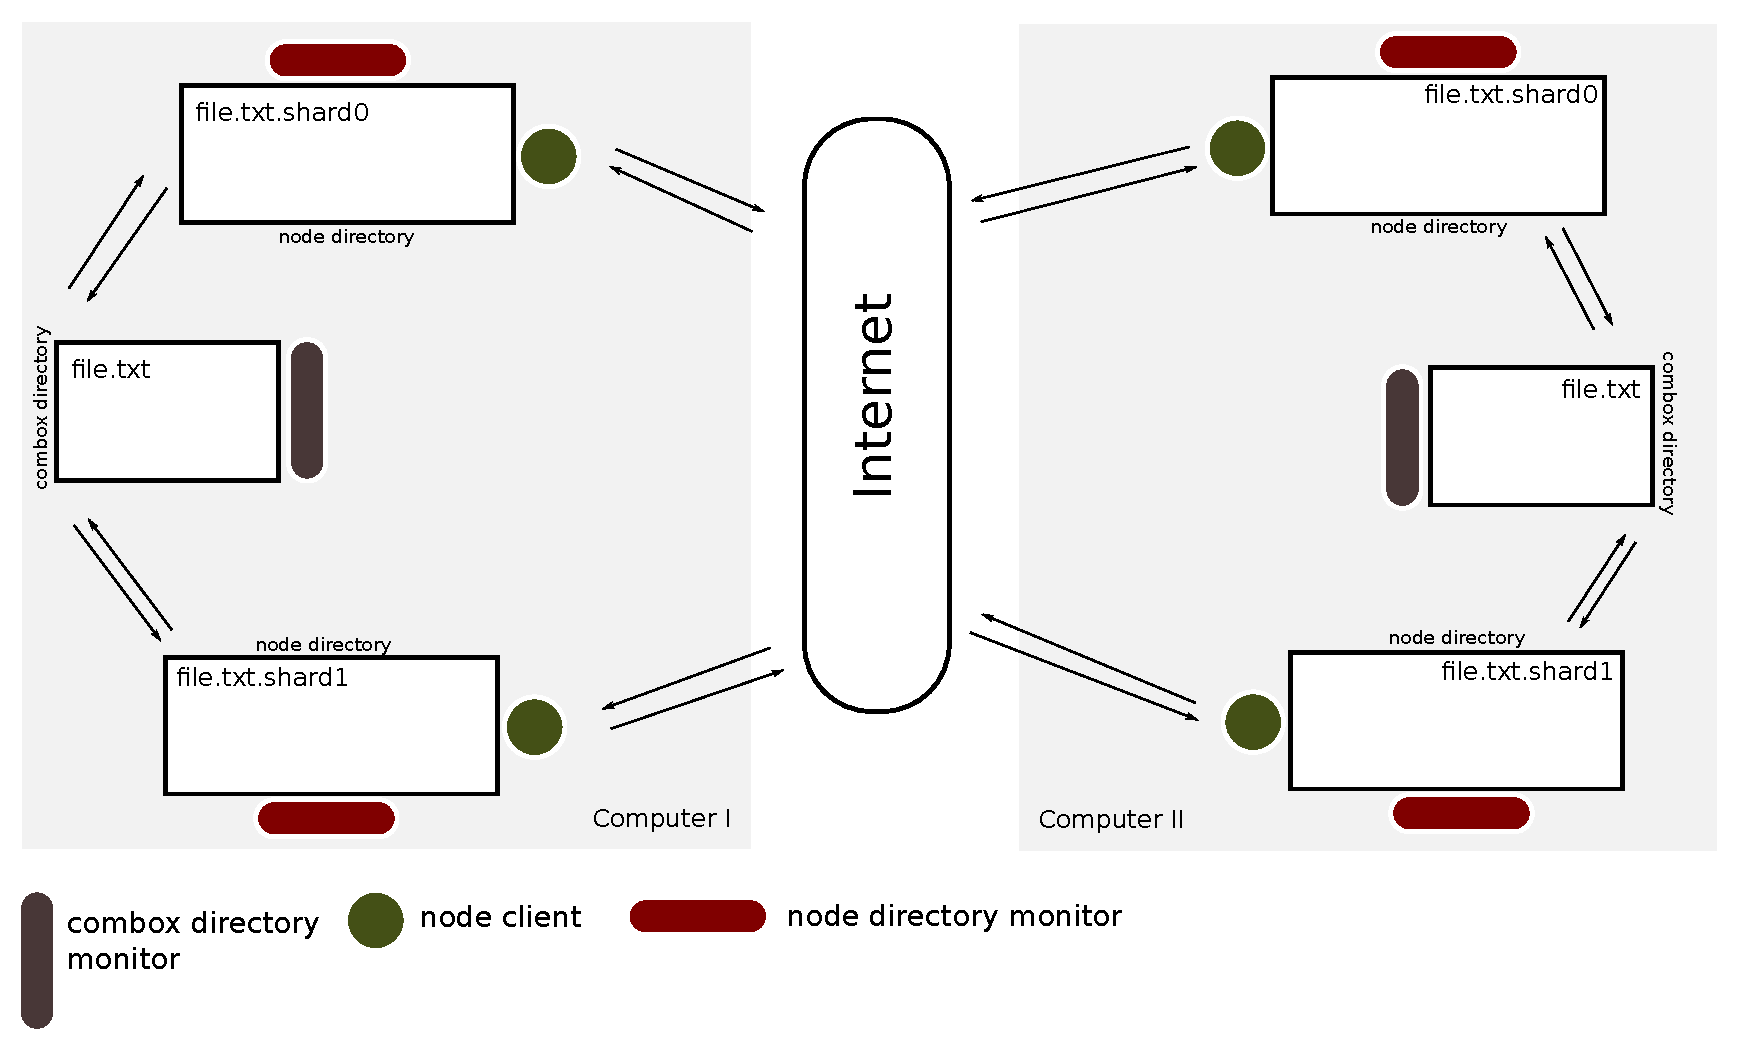
\includegraphics[scale=0.6]{4-combox-structure}
\caption{High level view of combox on two computers.}
\label{fig:4-combox-structure}
\end{figure}

\subsection{combox configuration}

\subsection{combox directory monitor}

\subsection{Node directory monitor}

\subsection{Database structure}

\section{combox modules overview}

combox is spread into modules that have functions and/or classes. As
of \verb+2016-02-04+ combox is considerably a small program:

\begin{verbatim}
$ wc -l combox/*.py
  144 combox/cbox.py
  178 combox/config.py
  241 combox/crypto.py
  891 combox/events.py
  541 combox/file.py
  454 combox/gui.py
    0 combox/__init__.py
   71 combox/log.py
  278 combox/silo.py
   29 combox/_version.py
 2827 total
\end{verbatim}

This section gives an overview of each of the combox modules with
extreme brevity:

\begin{description}
\item[combox.cbox] This module contains \verb+run_cb+ function runs
  combox; it creates an instance \verb+threading.Lock+ for database
  access and a shared \verb+threading.Lock+ for the
  \verb+combox.events.ComboxDirMonitor+ and
  \verb+combox.events.NodeDirMonitor+; it initializes an instance
  \verb+combox.events.ComboxDirMonitor+ that monitors the combox
  directory and an instance of \verb+combox.events.NodeDirMonitor+ for
  each node directory for monitoring the node directories. This
  modules also houses the \verb+main+ function that parses commandline
  arguments, starts combox configuration if needed or loads the combox
  configuration file to start running combox.
\item[combox.config] Accomodates two import functions --
  \verb+config_cb+ and \verb+get_nodedirs+. The \verb+config_cb+ is
  the combox configuration function that allows the user to configure
  combox; this function was designed in a such way that it was
  possible to use for both CLI and GUI methods of configuring
  combox. The \verb+get_nodedirs+ function returns, as a list, the
  paths of the node directories; this function use used in numerous
  places in other combox modules.
\item[combox.crypto] This has functions for encrypting and decrypting
  data; encrypting and decrypting shards (\verb+encrypt_shards+ and
  \verb+decrypt_shards+); a function for splitting a file into shards,
  encrypting those shards and spreading them across node directories
  (\verb+split_and_encrypt+); a function for decrypting the shards
  from the node directories, reconstructing the file from the
  decrypted shards and put the file back to the combox directory
  (\verb+decrypt_and_glue+). Functions \verb+split_and_encrypt+ and
  \verb+decrypt_and_glue+ are the two functions that that are
  extensively used by the \verb+combox.events+ module; all other
  functions in this module are pretty much helper functions are
  \verb+split_and_encrypt+ and \verb+decrypt_and_glue+ functions and
  are not used by other modules.
\item[combox.events] This module took the most time to write and test
  and it is the most complex module in combox at the time of writing
  this report. It contains just two classes -- \verb+ComboxDirMonitor+
  and \verb+NodeDirMonitor+. The \verb+ComboxDirMonitor+ inherits the
  \verb+watchdog.events.LoggingEventHandler+ and is responsible for
  monitoring for changes in the combox directory and doing the right
  thing when change happens in the combox directory. The
  \verb+NodeDirMonitor+ also inherits
  \verb+watchdog.events.LoggingEventHandler+ and similarly responsible
  for monitoring a node directory and doing the right thing when a
  change happens in the node directory; subjectively,
  \verb+NodeDirMonitor+ is slightly more complex than the
  \verb+ComboxDirMonitor+.
\item[combox.file] This is the second largest module in combox. It
  contains utility functions for reading, writing, moving
  files/directiores, hashing files, splitting a file into shards, glue
  shards into a file, manipulating directories inside combox and node
  directories.
\item[combox.gui] Contains the \verb+ComboxConfigDialog+ class; it is
  the graphical interface for configuring combox. The class uses the
  Tkinter library\cite{pylib:tkinter} for spawing graphical
  elements. Other graphical libraries include PyQt\cite{pylib:qt}
  were considered Tkinter was chosen over others because it works on
  all Unix systems and Microsoft's Windows and it is part of the core
  python (version 3).
\item[combox.log] All the messages to \verb+stdout+ and \verb+stderr+
  are sent through the functions \verb+log_i+ and \verb+log_e+
  functions defined in this module.
\item[combox.silo] Contains the \verb+ComboxSilo+ class which is the
  canonical interface for combox for managing information about the
  files in the combox directory. Internally, the \verb+ComboxSilo+
  class uses the pickleDB library\cite{pylib:pickledb}.
\item[combox.\_version] This is \emph{private} module that contains
  variables that contain the value of the present version and release
  of combox. The \verb+get_version+ function in this module returns
  the full version number; this function used by \verb+setup.py+.
\end{description}

\section{Language choice}

Back in October of 2014, I was learning to write in python and when I
had to start working on combox, I chose to write combox in python. In
my first commit to the combox repository, I had say say this about
python:

\begin{verbatim}
commit 2def977472b2e77ee88c9177f2d03f12b0263eb0
Author: rsiddharth <rsiddharth@ninthfloor.org>
Date:   Wed Oct 29 23:24:58 2014 -0400

    Initial commit: File splitter & File gluer done.

    ...

    I like to write python FWIW. But after reading a dialect of Lisp when
    I come back to python, it does not look very beautiful. I guess I'm
    pretty convinced that there is no language that can ape the beauty of
    Lisp.
\end{verbatim}

If I were to write that commit message today (\verb+2016-02-04+), I
would've phrased my reflections about python differently. While I've
not found a language that is as intrinsically beautiful as Lisp, I'm
not sure if it is not quite right to compare Lisp and Python. Python
is a very readable language and it tends to be very accessible to
beginners. Also, it is hard to write unreadable Python code.

\section{DRY}

The core functionality of combox is to split, encrypt file shards,
spread them across node directories (Google Drive and Dropbox) and
decrypt, glue shards and put them back to the combox directory when a
file is created/modified/deleted/moved in another computer. The plan
was to use external libraries to accomplish things fell outside the
realm of what I consider the ``core functionality of combox''; the
main reason behind this decision was to duly be an indolent programmer
and not indulge in trying to solve problems that others have already
solved.

The \verb+watchdog+\cite{pylib:watchdog} library used for file
monitoring; this library is compatible with Unix systems and
Windows. The \verb+pycrypto+ library\cite{pylib:pycrypto} was used for
encrypting data; combox uses AES encryption scheme to encrypt file
shards. The \verb+pickleDB+ library was used to store information
about files in the combox directory; this library is not very clean
but it was what I exactly looking for, if there was no
\verb+pickleDB+, I would've most probably written something similar to
it and made it as part of combox.

Looking back, the decision to use external libraries reduced the
complexity of combox, reduced the time to complete the initial working
version of combox and made it possible to spend more than 3 months
just testing and fixing issues in combox.

\section{Operating system compatibility}\label{4-os-compat}

\section{combox as a python package}

\section{With the benefit of hindsight}